\documentclass[12pt]{article}

\usepackage{sbc-template}

\usepackage{graphicx,url}

\usepackage[brazil]{babel}   
%\usepackage[latin1]{inputenc}  
\usepackage[utf8]{inputenc}  
% UTF-8 encoding is recommended by ShareLaTex

     
\sloppy

\title{Viabilidade do Uso Prático de Análise de Mutantes em Python}

\author{Sérgio Oliveira Campos\inst{1}, Ellen Francine Barbosa\inst{1}}

\address{Instituto de Ciências Matemáticas e Computação (ICMC) -- Universidade de São Paulo
  (USP)\\
  Avenida Trabalhador São-carlense, 400 - Centro -- 13566-590 -- São Carlos -- SP -- Brazil
  \email{seocam@usp.br, francine@icmc.usp.br}
}

\begin{document} 

\maketitle

\begin{abstract}
  This meta-paper describes the style to be used in articles and short papers
  for SBC conferences. For papers in English, you should add just an abstract
  while for the papers in Portuguese, we also ask for an abstract in
  Portuguese (``resumo''). In both cases, abstracts should not have more than
  10 lines and must be in the first page of the paper.
\end{abstract}
     
\begin{resumo} 
  Este meta-artigo descreve o estilo a ser usado na confecção de artigos e
  resumos de artigos para publicação nos anais das conferências organizadas
  pela SBC. É solicitada a escrita de resumo e abstract apenas para os artigos
  escritos em português. Artigos em inglês deverão apresentar apenas abstract.
  Nos dois casos, o autor deve tomar cuidado para que o resumo (e o abstract)
  não ultrapassem 10 linhas cada, sendo que ambos devem estar na primeira
  página do artigo.
\end{resumo}


\section{Introdução}


Análise de mutantes (ou teste de mutação) \cite{DeMillo:1978} é uma técnica 
utilizada para avaliar a qualidade de um conjunto de casos de teste. 
A técnica consiste
na alteração proposital de pequenos trechos de códigos afim de introduzir erros na
execução do programa. Apenas uma alteração é realizada por vez e os casos
de teste são executados novamente para cada uma das versões alteradas do
programa, denominadas mutantes.

Se ao menos um caso de teste fizer o programa
mutante se comportar de forma diferente do programa original, o mutante é dito 
``morto''. Quando um mutante tem comportamento comprovadamente idêntico ao 
programa original, o mutante não poderá ser morto e, neste caso, o mutante é
chamado de ``equivalente''. Cada alteração realizada no programa original é 
feita programaticamente através de
rotinas pré-determinadas. Estas rotinas, chamadas de operadores de mutação, variam
de acordo com cada linguagem.

Estudos realizados \cite{Frankl:1993, Li:2009, Andrews:2005} apontam que
o uso da análise de mutantes é mais efetiva do que outros critérios de 
cobertura em termos de detecção de falha; Devido ao alto custo da técnica
\cite{Gopinath:2014} chegou a conclusão que, na prática, o critério 
mais adequado para ser utilizado por desenvolvedores seria o de ``cobertura
de nós''. Em \cite{Li:2015}, relatam seus estudos sobre os desafios de se 
utilizar a análise de mutantes na prática com a linguagem Ruby, e chegam
a conclusão de que com adaptações na ferramenta testada (muRuby) a adoção
do critério seria viável.

Este artigo visa levantar quais são os fatores limitantes para o uso da análise
de mutantes durante o desenvolvimento de projetos Python reais.


\section{Análise de Mutantes em Python}

O Python é uma linguagem de programação de auto-nível, interpretada e de tipagem
dinâmica criada em 1991 por Guido Van Rossum e atualmente é mantida pela 
Python Software Foundation\footnotemark. Sua implementação de referência é o 
interpretador CPython escrito na linguagem C.

\footnotetext{Python Software Foundation -- https://www.python.org/}

Nessa seção será introduzido o estado atual da análise de mutantes na
linguagem Python.

\subsection{Mutantes Incompetentes}

Pelo fato de ser uma linguagem de tipagem dinâmica o interpretador Python não
é capaz de saber o tipo de uma determinada variável até o momento de sua
atribuição. Além disso o tipo de uma variável também pode ser alterado durante a 
execução do programa dentro de um mesmo escopo.

Por este motivo, o processo de criação de mutantes em Python estaria 
suscetível a gerar um maior número de mutantes com falhas consideradas
graves \cite{Bessam:2014}, que encerram a execução do programa antes do 
esperado, e por isso não são úteis na detecção de falhas no programa testado.
Este tipo de mutantes são chamados mutantes incompetentes \cite{Bottaci:2010}.

\subsection{Operadores de Mutação Suportados}

O potencial para geração de mutantes incompetentes é um problema para
a utilização de operadores de mutação propostos para outras linguagens,
além de limitar a criação de novos operadores. Hoje a linguagem Python conta com 20 operadores
de mutação, descritos por \cite{Derezinska:2014} e implementados na ferramenta
\textit{MutPy}\footnotemark, são estes:

\renewcommand{\labelitemi}{}
\begin{itemize}
    \item \textit{AOD} - arithmetic operator deletion
    \item \textit{AOR} - arithmetic operator replacement
    \item \textit{ASR} - assignment operator replacement
    \item \textit{BCR} - break continue replacement
    \item \textit{COD} - conditional operator deletion
    \item \textit{COI} - conditional operator insertion
    \item \textit{CRP} - constant replacement
    \item \textit{DDL} - decorator deletion
    \item \textit{EHD} - exception handler deletion
    \item \textit{EXS} - exception swallowing
    \item \textit{IHD} - hiding variable deletion
    \item \textit{IOD} - overriding method deletion
    \item \textit{IOP} - overridden method calling position change
    \item \textit{LCR} - logical connector replacement
    \item \textit{LOD} - logical operator deletion
    \item \textit{LOR} - logical operator replacement
    \item \textit{ROR} - relational operator replacement
    \item \textit{SCD} - super calling deletion
    \item \textit{SCI} - super calling insert
    \item \textit{SIR} - slice index remove
\end{itemize}


A linguagem C e a linguagem Ruby, por exemplo, contam com 71 \cite{Delamaro:1996} e 
54 operadores respectivamente \cite{Li:2015} (implementados nas 
ferramentas \textit{PROTEUM} e \textit{muRuby}).

\subsection{Ferramentas Python para Análise de Mutantes}


\footnotetext{MutPy -- https://bitbucket.org/khalas/mutpy}


\section{Trabalhos Relacionados}

\subsection{Aplicação Prática de Análise de Mutantes}

\section{Metodologia}

PATCH DO MUTPY

PROJETOS TESTADOS

PARAMETROS

\section{Dificuldades}

PORQUE O PATCH FOI PRECISO

TEMPO DE EXECUÇÃO

\section{Resultados}

TABELA

PROBLEMAS EM MUTANTES ENCONTRADOS (FALSOS TIMEOUTS e INCOMPETENTES)

PROBLEMAS DE CONFLITOS COM O MOCK

VELOCIDADE DA COBERTURA

\sections{AMEAÇAS A VALIDADE}

O PATCH APLICADO PODE TER AFETADO O FUNCIONAMENTO.

\section{Conclusões}

AS FERRAMENTAS PYTHON AINDA NÃO ESTÃO PRONTAS PARA USO EM AMBIENTES REAIS








\section{Figures and Captions}\label{sec:figs}


Figure and table captions should be centered if less than one line
(Figure~\ref{fig:exampleFig1}), otherwise justified and indented by 0.8cm on
both margins, as shown in Figure~\ref{fig:exampleFig2}. The caption font must
be Helvetica, 10 point, boldface, with 6 points of space before and after each
caption.

\begin{figure}[ht]
\centering
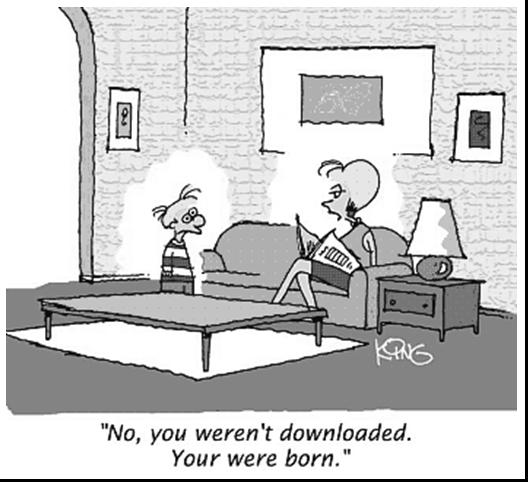
\includegraphics[width=.5\textwidth]{fig1.jpg}
\caption{A typical figure}
\label{fig:exampleFig1}
\end{figure}

\begin{figure}[ht]
\centering
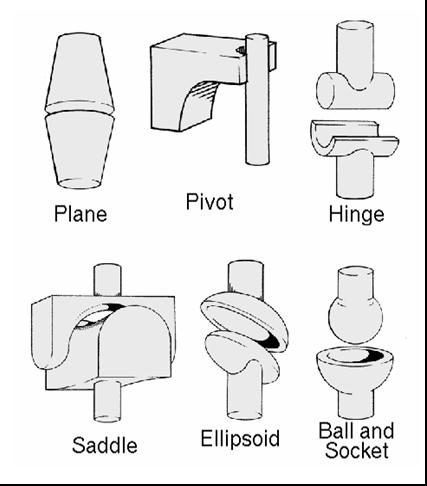
\includegraphics[width=.3\textwidth]{fig2.jpg}
\caption{This figure is an example of a figure caption taking more than one
  line and justified considering margins mentioned in Section~\ref{sec:figs}.}
\label{fig:exampleFig2}
\end{figure}

In tables, try to avoid the use of colored or shaded backgrounds, and avoid
thick, doubled, or unnecessary framing lines. When reporting empirical data,
do not use more decimal digits than warranted by their precision and
reproducibility. Table caption must be placed before the table (see Table 1)
and the font used must also be Helvetica, 10 point, boldface, with 6 points of
space before and after each caption.

\begin{table}[ht]
\centering
\caption{Variables to be considered on the evaluation of interaction
  techniques}
\label{tab:exTable1}
\smallskip
\begin{tabular}{|l|c|c|}
\hline
& Value 1 & Value 2\\[0.5ex]
\hline
&&\\[-2ex]
Case 1 & 1.0 $\pm$ 0.1 & 1.75$\times$10$^{-5}$ $\pm$ 5$\times$10$^{-7}$\\[0.5ex]
\hline
&&\\[-2ex]
Case 2 & 0.003(1) & 100.0\\[0.5ex]
\hline
\end{tabular}
\end{table}

\section{Images}

All images and illustrations should be in black-and-white, or gray tones,
excepting for the papers that will be electronically available (on CD-ROMs,
internet, etc.). The image resolution on paper should be about 600 dpi for
black-and-white images, and 150-300 dpi for grayscale images.  Do not include
images with excessive resolution, as they may take hours to print, without any
visible difference in the result. 


\bibliographystyle{sbc}
\bibliography{sbc-template}

\end{document}
